\documentclass[12pt]{report}
\usepackage[utf8]{inputenc}
\usepackage[english, russian]{babel}
\usepackage{listings}
\usepackage{graphicx}
\usepackage{float}
\graphicspath{{imgs/}}
\usepackage{amsmath,amsfonts,amssymb,amsthm,mathtools} 
\usepackage{pgfplots}
\usepackage{filecontents}
\usepackage{indentfirst}
\usepackage{eucal}
\usepackage{enumitem}
\frenchspacing

\usepackage{indentfirst} % Красная строка

\usetikzlibrary{datavisualization}
\usetikzlibrary{datavisualization.formats.functions}

\usepackage{amsmath}
\usepackage{fixltx2e}
\usepackage{caption}


\definecolor{bluekeywords}{rgb}{0,0,1}
\definecolor{greencomments}{rgb}{0,0.5,0}
\definecolor{redstrings}{rgb}{0.64,0.08,0.08}
\definecolor{xmlcomments}{rgb}{0.5,0.5,0.5}
\definecolor{types}{rgb}{0.17,0.57,0.68}

\usepackage{listings}
\lstset{language=[Sharp]C,
	captionpos=t,
	numbers=left, %Nummerierung
	numberstyle=\small, % kleine Zeilennummern
	frame=single, % Oberhalb und unterhalb des Listings ist eine Linie
	stepnumber=1,                   
	numbersep=5pt,                
	showspaces=false,
	tabsize=2,
	showtabs=false,
	breaklines=true,
	showstringspaces=false,
	breakatwhitespace=true,
	escapeinside={(*@}{@*)},
	commentstyle=\color{greencomments},
	morekeywords={partial, var, value, get, set},
	keywordstyle=\color{bluekeywords},
	stringstyle=\color{redstrings},
	basicstyle=\ttfamily\small,
}

\usepackage[left=2cm,right=2cm, top=2cm,bottom=2cm,bindingoffset=0cm]{geometry}
% Для измененных титулов глав:
\usepackage{titlesec, blindtext, color} % подключаем нужные пакеты
\definecolor{gray75}{gray}{0.75} % определяем цвет
\newcommand{\hsp}{\hspace{20pt}} % длина линии в 20pt
% titleformat определяет стиль
\titleformat{\chapter}[hang]{\Huge\bfseries}{\thechapter\hsp\textcolor{gray75}{|}\hsp}{0pt}{\Huge\bfseries}

\usepackage{array}
\newcommand{\head}[2]{\multicolumn{1}{>{\centering\arraybackslash}p{#1}}{#2}}

% plot
\usepackage{pgfplots}
\usepackage{filecontents}
\usetikzlibrary{datavisualization}
\usetikzlibrary{datavisualization.formats.functions}

\begin{document}
%\def\chaptername{} % убирает "Глава"
\thispagestyle{empty}
\begin{titlepage}
	\noindent \begin{minipage}{0.15\textwidth}
		
\includegraphics[width=\linewidth]{b_logo}
	\end{minipage}
	\noindent\begin{minipage}{0.9\textwidth}\centering
		\textbf{Министерство науки и высшего образования Российской Федерации}\\
		\textbf{Федеральное государственное бюджетное образовательное учреждение высшего образования}\\
		\textbf{~~~«Московский государственный технический университет имени Н.Э.~Баумана}\\
		\textbf{(национальный исследовательский университет)»}\\
		\textbf{(МГТУ им. Н.Э.~Баумана)}
	\end{minipage}
	
	\noindent\rule{18cm}{3pt}
	\newline\newline
	\noindent ФАКУЛЬТЕТ $\underline{\text{«Информатика и системы управления»}}$ \newline\newline
	\noindent КАФЕДРА $\underline{\text{«Программное обеспечение ЭВМ и информационные технологии»}}$\newline\newline\newline\newline\newline\newline\newline\newline\newline\newline\newline
	
	
	\begin{center}
		\noindent\begin{minipage}{1.3\textwidth}\centering
			\Large\textbf{  Отчет по лабораторной работе №7}\newline
			\textbf{по дисциплине "Анализ алгоритмов"}\newline\newline
		\end{minipage}
	\end{center}
	
	\noindent\textbf{Тема} $\underline{\text{Поиск в словаре}}$\newline\newline
	\noindent\textbf{Студент} $\underline{\text{Малышев И. А.}}$\newline\newline
	\noindent\textbf{Группа} $\underline{\text{ИУ7-51Б}}$\newline\newline
	\noindent\textbf{Оценка (баллы)} $\underline{\text{~~~~~~~~~~~~~~~~~~~~~~~~~~~}}$\newline\newline
	\noindent\textbf{Преподаватель: } $\underline{\text{Волкова Л. Л.}}$\newline\newline\newline
	
	\begin{center}
		\vfill
		Москва~---~\the\year
		~г.
	\end{center}
\end{titlepage}


\renewcommand{\contentsname}{Содержание}
\tableofcontents
\setcounter{page}{2}

\newpage
\chapter*{Введение}
\addcontentsline{toc}{chapter}{Введение}

Словарь  -- структура данных, построенная  на  основе  пар  значений: ключ-значение.  Ключ нужен для идентификации элементов, а значение -- это собственно сам хранимый элемент. Например, в телефонном справочнике номеру  телефона  соответствует  фамилия  абонента. Существует несколько основных различных реализаций словаря: массив, двоичные деревья поиска, хеш-таблицы. Каждая из этих реализаций имеет свои минусы и плюсы, например время поиска, вставки и удаления элементов.

\textbf{Целью} данной лабораторной работы является изучение, реализация и сравнение алгоритмов поиска в словаре.

В рамках выполнения работы необходимо решить следующие \textbf{задачи}:

\begin{itemize}
	\item реализовать три алгоритма поиска в словаре: линейный, бинарный и поиск с частотным анализом;
	\item замерить количество сравнений при поиске и сравнить данные между алгоритмами;
	\item сделать выводы на основе проделанной работы.
\end{itemize}

\chapter{Аналитическая часть}

В данном разделе представленные теоретические сведения о рассматриваемых алгоритмах.

\section{Полный перебор}

Алгоритм полного перебора заключается в проходе по словарю, до того момента, пока не будет найден искомый ключ. В рассматриваемом алгоритме возможно $N + 1$ случаев расположения ключа: ключ является $i$-ым элементом словаря либо его нет в словаре в принципе. 

Лучший случай (трудоемкость $O(1)$): ключ расположен в самом начале словаря и найден за одно сравнение). Худший случай (трудоемкость $O(N)$): ключ расположен в самом конце словаря либо ключ не находится в словаре.

\section{Двоичный поиск}

Данный алгоритм подходит только для заранее упорядоченного словаря.

Процесс двоичного поиска можно описать следующим образом: 

\begin{itemize}
	\item получить значение находящееся в середине словаря и сравнить его с ключом;
	\item в случае, если ключ меньше данного значения, продолжить поиск в младшей части словаря, в обратном случае -- в старшей части словаря;
	\item на новом интервале снова получить значение из середины этого интервала и сравнить с ключом.
	\item поиск продолжать до тех пор, пока не будет найден искомый ключ, или интервал поиска не окажется пустым.
\end{itemize}

Обход словаря данным алгоритм можно представить в виде дерева, поэтому трудоемкость в худшем случае составит $\log_{2}{N}$. Можно сделать вывод, что алгоритм двоичного поиска работает быстрее чем алгоритм полного перебора, но при этом требует предварительной обработки данных (сортировки)\cite{levitin}.

\section{Частотный анализ}

Данный алгоритм также требует предварительной обработки данных, а именно:

\begin{itemize}
	\item упорядочить словарь;
	\item разбить словарь на сегменты (сегментация).
\end{itemize}

Словарь разбивается на сегменты по какому-либу признаку и сортируется по частоте. Например, если ключ является строкой, то можно сделать разбиение по первой букве в ключе. Если ключ является целым числом, можно провести разбиение по остатку от деления ключа на некоторое число $K$.

После выполнения разбиения, нужно определить к какому сегменту относится искомый ключ и провести на этом сегменте двоичный поиск.

Таким образом, время поиска в словаре увеличивается (особенно для самых часто встречаемых ключей), но, при этом, так же как и алгоритм двоичного поиска, частотный анализ требует предварительной обработки данных (сортировки и сегментации)\cite{koutiho}. 

\section{Описание словаря}

Ключом в рассматриваемом мною словаре является Имя персонажа из книги <<Божественная комедия>>\cite{dante}, а значением -- его описание. Оба значения являются строковыми. Так как значение ключа является строкой, деление на сегменты будет производится посредством получения первой буквы в ключе.

\section*{Вывод}
В данном разделе были рассмотренны особенности алгоритмов поиска в словаре.

\chapter{Конструкторская часть}

В данном разделе представлены схемы рассматриваемых алгоритмов.

\section{Разработка алгоритмов}

На рисунках 2.1 - 2.3 приведены схема алгоритмов поиска в словаре.

\begin{figure}[H]
	\centering
	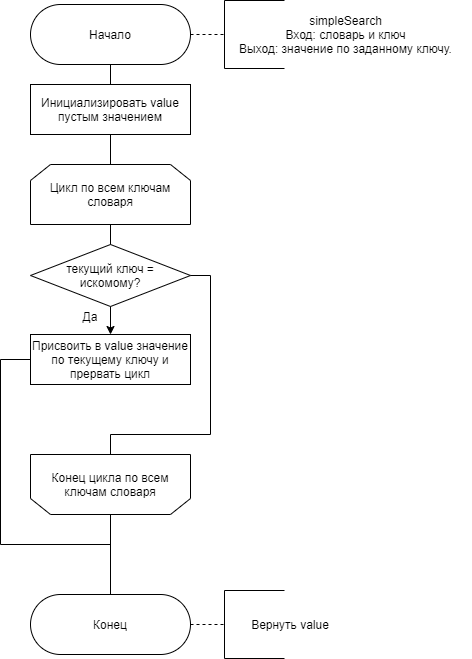
\includegraphics[scale=0.8]{simple_search.drawio.png}
	\caption{Схема алгоритма полного перебора.}
	\label{fig:mpr}
\end{figure}

\begin{figure}[H]
	\centering
	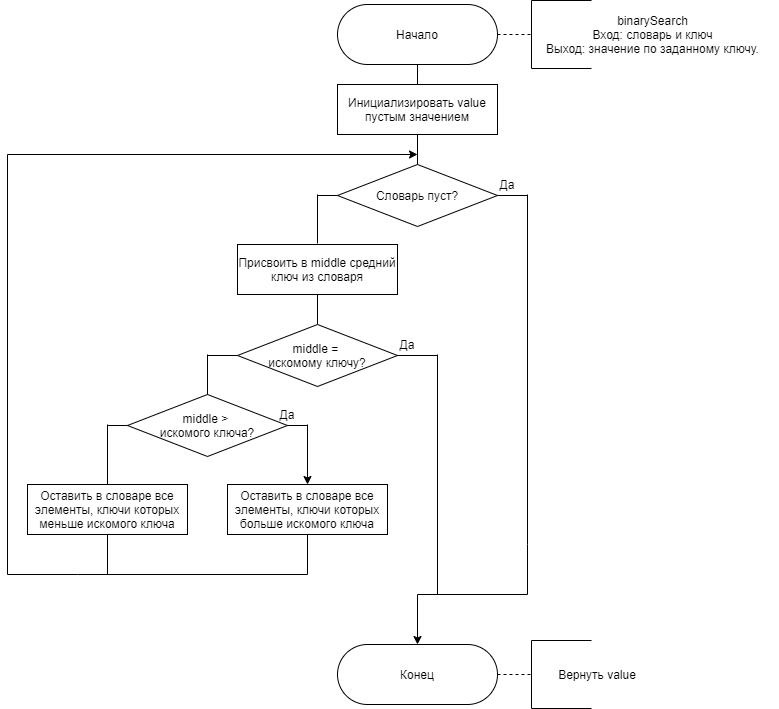
\includegraphics[scale=0.7]{binary_search.drawio.png}
	\caption{Схема алгоритма двоичного поиска.}
	\label{fig:mpr}
\end{figure}

\begin{figure}[H]
	\centering
	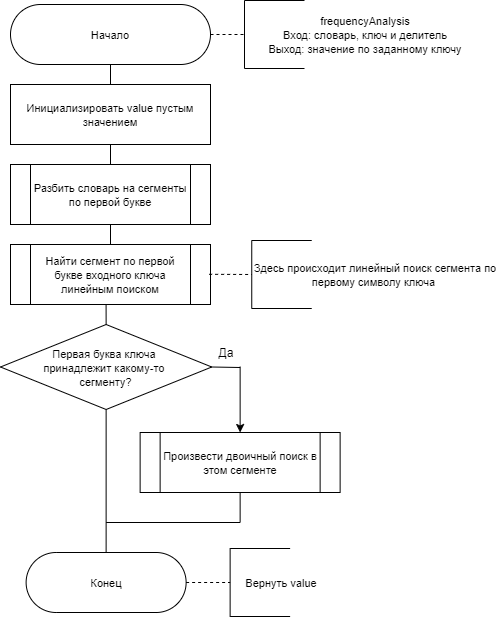
\includegraphics[scale=0.8]{freq_analysis.drawio.png}
	\caption{Схема алгоритма поиска с использованием частотного анализа.}
	\label{fig:mpr}
\end{figure}


\section*{Вывод}

На основе теоретических данных, полученных аз аналитического раздела, были построенны схемы алгоритмов поиска в словаре.

\chapter{Технологическая часть}

В данном разделе приведены средства реализации и листинги кода.

\section{Средства реализации}

В качестве языка программирования был выбран C\# \cite{Microsoft}, а среды разработки -- Visual Studio\cite{VS}, т. к. я знаком с данным языком и имею представление о тестировании программ в данном языке.

\section{Реализация алгоритмов}

В листингах 3.1 - 3.3 представлены листинги алгоритмов поиска в словаре.

\captionsetup{singlelinecheck = false, justification=raggedright}
\begin{lstlisting}[label=some-code,caption=Алгоритм полного перебора]
public string LinearSearch(string key, out int cmp_cnt)
{
	cmp_cnt = 0;
	foreach (var d in dict)
	{
		cmp_cnt++;
		if (d.Key == key)
			return d.Value;
	}
	
	return null;
}
\end{lstlisting}

\newpage
\begin{lstlisting}[label=some-code,caption=Алгоритм двоичного поиска]
public string BinarySearch(string key, int left, int right, out int cmp_cnt)
{
	int cmp, mid;
	cmp_cnt = 0;
	
	while (left <= right)
	{
		mid = left + (right - left) / 2;
		
		cmp_cnt++;
		if ((cmp = key.CompareTo(this[mid].Key)) > 0)
			left = mid + 1;
		else if (cmp < 0)
			right = mid - 1;
		else
			return dict[mid].Value;
	}
	
	return null;
}
\end{lstlisting}

\begin{lstlisting}[label=some-code,caption=Алгоритм поиска с использованием частотного анализа]
public void Clusterize()
{
	for (int i = 0; i < dict.Count; i++)
	{
		string key = dict[i].Key[0].ToString();
		if (clusters.ContainsKey(key))
			clusters[key] = new KeyValuePair<int, int>(Math.Min(clusters[key].Key, i), Math.Max(clusters[key].Value, i));
		else
			clusters.Add(key, new KeyValuePair<int, int>(i, i));
	}
}

public string ClusterSearch(string key, out int cmp_cnt)
{
	string cluster_key = key[0].ToString();
	return BinarySearch(key, clusters[cluster_key].Key, clusters[cluster_key].Value, out cmp_cnt);
}
\end{lstlisting}
\captionsetup{singlelinecheck = false, justification=centering}

\section{Результаты тестирования}

В таблице 3.1 приведены тестовые данные, где ПП -- полный перебор, ДП -- двоичный поиск, ЧА -- частотный анализ. Все тесты были пройденны успешно.

\begin{table}[H]
	\caption{Таблица тестовых данных алгоритмов поиска в словаре.}
	
	\begin{center}
		
		\begin{tabular}{|c c c c c|} 
			
			\hline
			
			Входные данные & Ожидаемый результат & ПП & ДП & ЧА \\  
			
			\hline
			
			Ahithophel & See Absalom & See Absalom & See Absalom & See Absalom \\
			
			\hline
			
			Michael & Archangel & Archangel & Archangel & Archangel \\
			
			\hline
			
			Ulysses & See Odysseus & See Odysseus & See Odysseus & See Odysseus \\
			
			\hline
			
			erhgrgher & null & null & null & null \\
			\hline
		\end{tabular}
		
	\end{center}
	
\end{table}

\section*{Вывод}

В данном разделе были разработаны и протестированны алгоритмы поиска в словаре.

\chapter{Исследовательская часть}

В данном разделе приведен анализ характеристик разработанного ПО.

\section{Результаты анализа}

На рисунках 4.1 - 4.5 приведены результаты анализа алгоритмов поиска в словаре. Индекс ключа -- положение ключа в словаре. Для случаев двоичного поиска и поиска с частотным анализом словари были приведены к требуемому виду.

\begin{figure}[H]
	\centering
	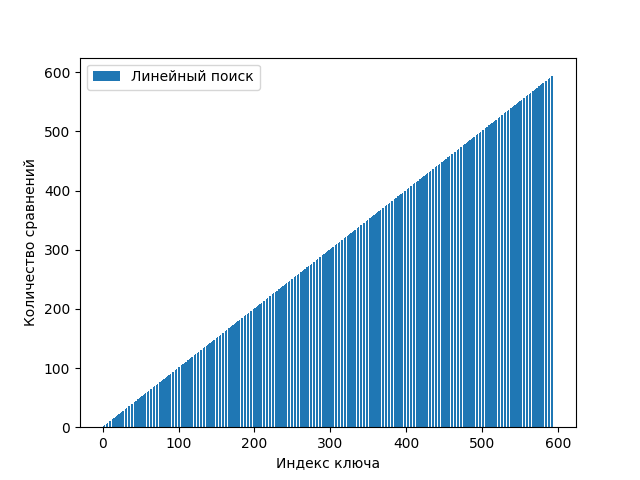
\includegraphics[scale=0.8]{lin_search.png}
	\caption{Анализ количества сравнений для линейного поиска.}
	\label{fig:mpr}
\end{figure}

\begin{figure}[H]
	\centering
	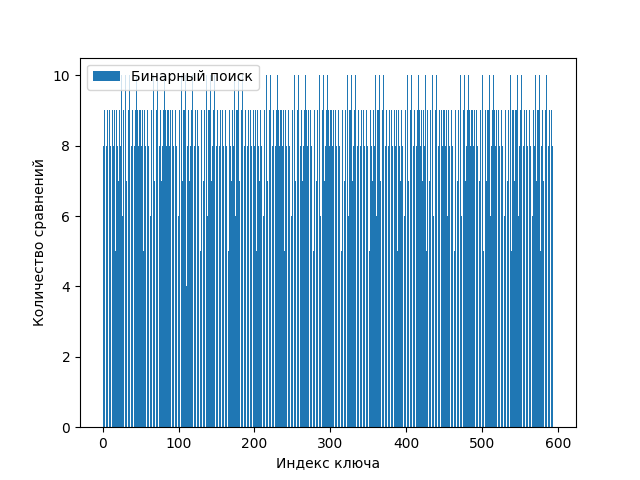
\includegraphics[scale=0.8]{bin_search.png}
	\caption{Анализ количества сравнений для двоичного поиска.}
	\label{fig:mpr}

\end{figure}

\begin{figure}[H]
	\centering
	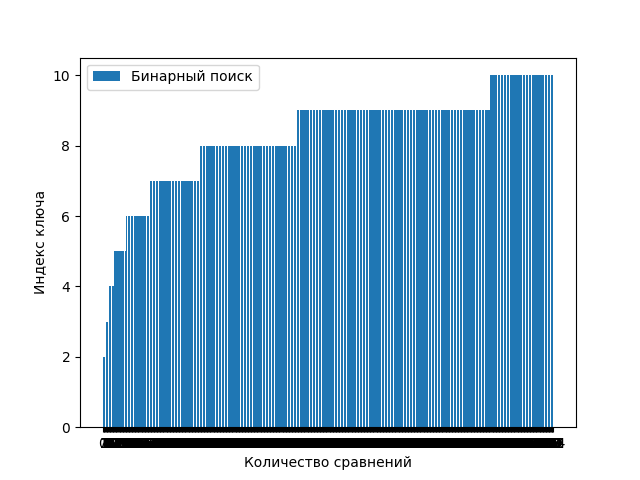
\includegraphics[scale=0.8]{bin_search_sorted.png}
	\caption{Анализ количества сравнений для двоичного поиска (отсортировано по количеству сравнений).}
	\label{fig:mpr}
\end{figure}

\begin{figure}[H]
	\centering
	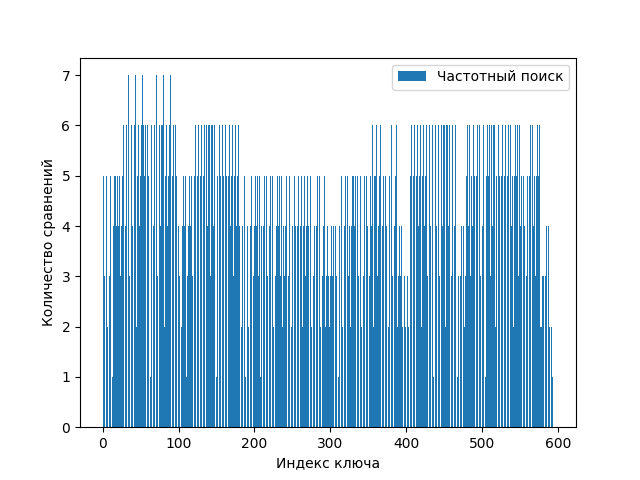
\includegraphics[scale=0.8]{clust_search.png}
	\caption{Анализ количества сравнений для поиска с использованием частотного анализа.}
	\label{fig:mpr}
\end{figure}

\begin{figure}[H]
	\centering
	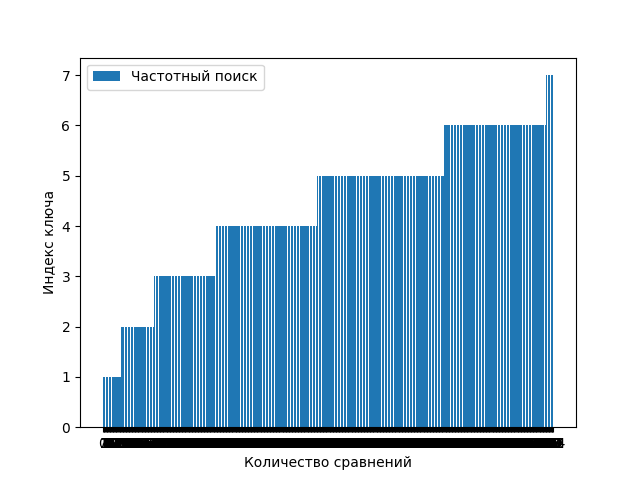
\includegraphics[scale=0.8]{clust_search_sorted.png}
	\caption{Анализ количества сравнений для поиска с использованием частотного анализа (отсортировано по количеству сравнений).}
	\label{fig:mpr}
\end{figure}

\section*{Вывод}

Алгоритм двоичного поиска превосходит алгоритм полного перебора для любово ключа в словаре. Количество сравнений в двоичном поиске не превышает $ceil(\log_{2}{n})$, где $n$ -- размер словаря, когда как в линейном -- линейно зависит от $n$. 

Алгоритм поиска с использованием частотного анализа выигрывает у алгоритма двоичного поиска, т. к. уменьшается количество сравнений из-за в заранее известного диапазона поиска. Количество сравнений в поиске с частотным анализом не превышает $ceil(\log_{2}{max(m)})$, где $m$ -- размер сегмента.

Минимальное возможное количество сравнений в словаре для всех алгоритмов одинаково и равно 1.

\chapter*{Заключение}
\addcontentsline{toc}{chapter}{Заключение}

В рамках данной лабораторной работы лабораторной работы была достигнута её цель: изучены алгоритмы поиска в словаре. Также выполнены следующие задачи:

\begin{itemize}
	\item реализованны три алгоритма поиска в словаре;
	\item замерено количество сравнений во время поиска для всех алгоритмов;
	\item сделаны выводы на основе проделанной работы.
\end{itemize}

В результате проведения сравнения количества сравнений алгоритмов, можно сделать вывод, что алгоритм поиска с использованием частотного анализа выигрывает у алгоритма двоичного поиска, т. к. уменьшается количество сравнений из-за в заранее известного диапазона поиска.

Стоит отметить, что и алгоритм двоичного поиска, и алгоритм поиска с использованием частотного анализа требуют предварительной обработки данных (сортировки и сегментации соотвественно), в отличие от алгоритма полного перебора. Но именно это позволяет стать этим алгоритмам намного эффективнее в сравнении с алгоритмом полного перебора, где количество сравнений линейно растёт от размера словаря.

Поставленная цель была достигнута.

\newpage
\addcontentsline{toc}{chapter}{Список литературы}
\renewcommand\bibname{Список литературы}
\begin{thebibliography}{3}
	\bibitem{levitin} Левитин А. В. Глава 4. Метод декомпозиции: Бинарный поиск // Алгоритмы. Введение в разработку и анализ — М.: Вильямс, 2006. — С. 180—183. — 576 с.
	\bibitem{koutiho} С.Коутинхо. Введение в теорию чисел. Алгоритм RSA. Москва: Постмаркет, 2001. — 328 с.
	\bibitem{dante} Данте Алигьери. Божественная комедия. Перевод М.Лозинского. ББК 84.4 Ит, Д 17, Издательство "Правда", М.: 1982, OCR Бычков М.Н.
	\bibitem{Microsoft} Руководство по языку C\#[Электронный ресурс], - режим доступа: https://docs.microsoft.com/ru-ru/dotnet/csharp/
	\bibitem{VS} Visual Studio[Электронный ресурс], - режим доступа: https://visualstudio.microsoft.com/ru/
\end{thebibliography}

\end{document}